\documentclass[a4paper,10pt]{article}

\usepackage[english]{babel}
\usepackage[utf8]{inputenc}
\usepackage{titlesec}
\usepackage{graphicx}
\usepackage{mathtools}
\usepackage{amsthm}
\usepackage{amsfonts}
\usepackage[top=1.0in,bottom=1.0in]{geometry}
\usepackage{hyperref}
\usepackage[singlelinecheck=false]{caption}
\usepackage[backend=biber,url=true,doi=true,eprint=false,style=alphabetic]{biblatex}
\usepackage{enumitem}
\usepackage[x11names, rgb]{xcolor}
\usepackage{tikz}
\usepackage[justification=centering]{caption}
\usepackage{indentfirst}
\usepackage{abstract}
\usepackage[titletoc]{appendix}
\usepackage{bookmark}

\usetikzlibrary{snakes,arrows,shapes}

\addbibresource{../common/references.bib}

\newcommand\blfootnote[1]{%
  \begingroup
  \renewcommand\thefootnote{}\footnote{#1}%
  \addtocounter{footnote}{-1}%
  \endgroup
}

\DeclareMathOperator*{\argmin}{arg\,min}
\DeclareMathOperator*{\argmax}{arg\,max}

\newcommand\defeq{\mathrel{\overset{\makebox[0pt]{\mbox{\normalfont\tiny\sffamily def}}}{=}}}

\renewcommand{\abstractnamefont}{\normalfont\Large\bfseries}

\titleformat{\section}
  {\normalfont\scshape\bfseries}{\thesection}{1em}{}
\titleformat{\subsection}
  {\normalfont\scshape\bfseries}{\thesubsection}{1em}{}
\titleformat{\paragraph}
  {\normalfont}{\theparagraph}{1em}{}
\titleformat{\subparagraph}
  {\normalfont}{\thesubparagraph}{1em}{}

\captionsetup[table]{labelsep=space}

\theoremstyle{plain}

\newtheorem*{spn-def}{Definition}
\newtheorem*{spn-thm}{Theorem}

\setlength{\parskip}{1em}

\begin{document}

\begin{titlepage}
  \begin{center}
    \LARGE
    \textbf{An Introduction to Sum-Product Networks}

    \vspace{1.7cm}
    \Large
    A collection of studies on properties, structure, inference and learning on Sum-Product
    Networks

    \vspace{1.7cm}
    \large
    Student: Renato Lui Geh

    Supervisor: Denis Deratani Mauá (DCC IME-USP)
    \vfill
    \large
    University of São Paulo / Universidade de São Paulo (USP)

    Institute of Mathematics and Statistics / Instituto de Matemática e Estatística (IME)
    \vspace{1.5cm}
  \end{center}
\end{titlepage}

\newpage
\null\vspace{\fill}
\begin{abstract}
  \large
  This work is a collection of ongoing studies I am working on for my undergraduate research
  project on automatic learning of Sum-Product Networks. The main objective of this work is logging
  my study notes on this subject in an instructive and uncomplicated way. Most scientific papers
  are cluttered with intricate names and require extensive background on the subject in order for
  the reader to understand what is going on. In this paper we seek to provide an easy reference and
  introductory reading material to those who intend to work with Sum-Product Networks.

  This study is divided into five main sections. We start with an introductory section regarding
  probabilistic graphical models and why Sum-Product Networks are so interesting. Next we talk
  about the structure of the model. Thirdly, we analyse some properties and theorems. Fourthly, we
  look on how to perform exact tractable inference. And finally we take a look at how to perform
  learning.
\end{abstract}
\vspace{\fill}
\newpage
\large
\tableofcontents
\normalsize
\newpage

\section{Introduction}

We assume the reader has already read the notation [Appendix~\ref{app:not}] and has the
mathematical background required [Appendix~\ref{app:bak}] defined in the Appendix.

In this section we show what the usual problems with probabilistic graphical models are and what
led to the creation of Sum-Product Networks. Additionally, we show some results from experiments
Poon and Domingos performed on the inaugural Sum-Product Network article \textit{Sum-Product
Networks: A New Deep Architecture}~\cite{poon-domingos}.

\subsection{Motivation}

Probabilistic Graphical Models (PGMs) perform inference through posterior probabilities on the
query and evidence. Thus, inference would look roughly like this:

\begin{equation*}
  P(X | \mathbf{e}=e_1,\ldots,e_q)
\end{equation*}

Where $X$ is called the variable query and $\mathbf{e}$ the evidence, that is, the observed
instances of the variables.

Using the definition of conditional probability,

\begin{equation*}
  P(X|\mathbf{e})=\frac{P(X,\mathbf{e})}{P(\mathbf{e})}
\end{equation*}

We get the following equation:

\begin{equation}
  P(X|\mathbf{e})=\frac{P(X,\mathbf{e})}{P(\mathbf{e})}=\alpha P(X,\mathbf{e})=\alpha
  \sum_{\mathbf{y}} P(X,\mathbf{e},\mathbf{y})
\end{equation}

Where $\mathbf{y}$ is a hidden variable. That is, let $\mathbf{X}$ be the complete set of
variables. Then $\mathbf{X}=\{X\} \cup \mathbf{E} \cup \mathbf{Y}$, where $X$ is the query,
$\mathbf{E}$ is the set of evidence variables and $\mathbf{Y}$ is a set of non-query non-evidence
variables. Thus $\mathbf{y}$ is an instance of $\mathbf{Y}$.

We can see that $P(X,\mathbf{e},\mathbf{y})$ is actually a subset of the full joint distribution.
Since we are summing out the hidden variables, we are actually discarding all the possible values
of $\mathbf{y}$ and taking into account all the possibilities where the query given the evidence
occur.

Now consider a Bayesian network as the PGM of our choice. We know that Bayesian networks have the
property of representing the full joint distribution as a product of conditional probabilities:

\begin{equation}
  P(x_1,\ldots,x_n) = \prod_{i=1}^n P(x_i|Par(X_i))
\end{equation}

Where $Par(X_i)$ are the values of the parents of $X_i$. From this property we know that we can
now compute inference by applying Equation (2) on Equation (1). By doing that we get inference by
computing the sum of products of conditional probabilities from the network. This is fundamental
to Adnan Darwiche's \textit{network polynomial}~\cite{diff-approach-darwiche,bayes-net-darwiche},
a concept that is the core of Sum-Product Networks.

We know that we can compute inference by summing out the hidden variables and then multiplying the
remaining factors, but this process relies on adding and then multiplying an exponential number of
probabilities. In fact, if we don't take the order of the terms in the summation into account, the
complexity reaches $O(np^n)$, where $p$ is the number of possible values a variable may take. If we
move the independent terms from the summation the complexity is then $O(p^n)$. This is obviously
intractable, and a reason why approximate inference is often the best solution.

Bayesian networks are not the only model that have intractable exact inference. Most PGMs suffer
from intractability of inference, and hence intractability of learning. However Domingos and Poon
argument that ``classes of graphical models where inference is tractable exist [\ldots], but are
quite limited in the distributions they can represent compactly.''~\cite{poon-domingos}.

Sum-Product Networks provide a graphical model where inference is both tractable and exact whilst
still being more general than existing tractable models.

\subsection{Background}

In Adnan Darwiche's \textit{A Differential Approach to Inference in Bayesian Networks}
\cite{diff-approach-darwiche} and \textit{Modeling and Reasoning with Bayesian Networks}
\cite{bayes-net-darwiche}, Darwiche presents a new way of representing full joint distributions
through a \textit{network polynomial}. In this subsection we will show what a network polynomial
is.

Consider the following Bayesian network:

\begin{figure}[h]
  \centering{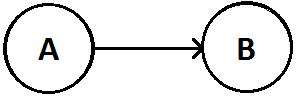
\includegraphics[scale=0.5]{imgs/bayes_net.png}
    \caption{A Bayesian network $A \to B$, that is, the variable $B$ depends on $A$.}
  }
\end{figure}

\begin{table}[h]
  \begin{center}
    \captionsetup{justification=centering}
    \begin{tabular}{c | c}
      A & $\Theta_A$ \\
      \hline
      $a$ & $\theta_a = 0.3$ \\
      $\overline{a}$ & $\theta_{\overline{a}} = 0.7$ \\
    \end{tabular}
    \quad
    \quad
    \begin{tabular}{c c | c}
      A & B & $\Theta_{B|A}$ \\
      \hline
      $a$ & $b$ & $\theta_{b|a}=0.1$ \\
      $a$ & $\overline{b}$ & $\theta_{\overline{b}|a}=0.9$ \\
      $\overline{a}$ & $b$ & $\theta_{b|\overline{a}}=0.8$ \\
      $\overline{a}$ & $\overline{b}$ & $\theta_{\overline{b}|\overline{a}}=0.2$ \\
    \end{tabular}
    \caption*{Tables 1 and 2}
  \end{center}
\end{table}
\setcounter{table}{2}

The two tables above describe the Bayesian network in Figure 1. From these tables we can construct
the full joint distribution table by applying the definition of conditional probability we saw in
the previous subsection.

\begin{table}[h]
  \begin{center}
    \captionsetup{justification=centering}
    \begin{tabular}{c c | c}
      A & B & $P(A,B)$ \\
      \hline
      $a$ & $b$ & $\theta_a\theta_{b|a}$ \\
      $a$ & $\overline{b}$ & $\theta_a\theta_{\overline{b}|a}$ \\
      $\overline{a}$ & $b$ & $\theta_{\overline{a}}\theta_{b|\overline{a}}$ \\
      $\overline{a}$ & $\overline{b}$ & $\theta_{\overline{a}}\theta_{\overline{b}|\overline{a}}$\\
    \end{tabular}
    \caption{The full joint distribution of the Bayesian network in Figure 1.}
  \end{center}
\end{table}

Before we proceed we need to understand the concept of variable indicators and their consistency
with their respective variables. We will take Boolean variables for simplicity as example. An
indicator of a variable, usually written as $[\cdot]$ has a value of $1$ if the variable is true
and value $0$ otherwise. Since $[X_i]$ is quite cumbersome, we abbreviate $[X_i]$ as $x_i$
and $[\overline{X}_i]$ as $\overline{x}_i$. See [Appendix~\ref{app:not}] with regards to
conflicting notations. Let us now define the notation of indicators more formally.

\begin{spn-def}
  Let $\mathbf{X}=\{X_1,\ldots,X_n\}$ be the set of all variables in Bayesian network
  $\mathcal{N}$, with each variable $X_i$ having $p$ possible values. Then the indicators of
  an arbitrary variable $X_i$ are denoted by $x_{i_j}$, $1\leq j \leq p$ where $j$ is the $j$-th
  possible value of the variable. All indicators follow the consistency rule.
\end{spn-def}

For $p=2$, we can abbreviate $x_{i_1}$ and $x_{i_2}$ to $x_i$ and $\overline{x}_i$ and consider
Boolean values. Let us now define consistency. We will define consistency for Boolean values. The
extension to multi-valued variables is not discussed here.

\begin{spn-def}
  Let $\mathbf{x}=\{x_1,\ldots,x_n,\overline{x}_1,\ldots,\overline{x}_n\}$ be the set of indicators
  of all variables in the set $\mathbf{X}=\{X_1,\ldots,X_n\}$, where variable $X_i$ may have values
  $1$ or $0$, with $x_i$ representing $1$ and $\overline{x}_i$ otherwise. Let $\mathbf{e}=\{e_p,
  \ldots,e_q\}$ be the set of an observed event as evidence where $e_j$ represents an observed
  value for variable $X_j$ in set $\overline{X}$. Then the set $\mathbf{X}$ is consistent with
  $\mathbf{e}$ iff:

  \begin{itemize}
    \item For each variable $X_i$ in set $\mathbf{X}$:
      \begin{itemize}
        \item If there exists an observed value $e_i$ in $\mathbf{e}$, then:
        \begin{itemize}
          \item If $e_i=1$, then $x_i=1$ and $\overline{x}_i=0$.
          \item If $e_i=0$, then $x_i=0$ and $\overline{x}_i=1$.
        \end{itemize}
        \item If there is no observed value $e_i$ for $X_i$, then:
        \begin{itemize}
          \item $x_i=1$ and $\overline{x}_i=1$.
        \end{itemize}
      \end{itemize}
  \end{itemize}
\end{spn-def}

We now introduce Darwiche's network polynomial. Darwiche, in his article and book
\cite{diff-approach-darwiche,bayes-net-darwiche}, uses indicators as $\lambda_i$ and
$\lambda_{\overline{i}}$ instead of $x_i$ and $\overline{x}_i$. However, they are exactly the same
as we have defined here. Since we named our variables $A$ and $B$ earlier, we will use Darwiche's
notation for just this example, since it's more readable. For other examples we will use our own
notation.

Table 3 is the full joint distribution that represents the Bayesian network in Figure 1. Darwiche
proposes a compact way to represent such distribution by taking each term in the joint
distribution, multiplying the relevant indicators, and then summing all terms into a polynomial
function. This function is named the network polynomial (Equation 3) of the Bayesian network.

\begin{equation}
  \Phi = \lambda_a\lambda_b\theta_a\theta_{b|a} +
      \lambda_a\lambda_{\overline{b}}\theta_a\theta_{\overline{b}|a} +
      \lambda_{\overline{a}}\lambda_b\theta_{\overline{a}}\theta_{b|\overline{a}} +
      \lambda_{\overline{a}}\lambda_{\overline{b}}\theta_{\overline{a}}\theta_{\overline{b}|\overline{a}}
\end{equation}

To compute the probability of any evidence $\mathbf{e}$, we compute $\Phi(\mathbf{e})$ such that
all indicators are consistent with $\mathbf{e}$. If we assume that the indicators will always be
consistent with the evidence, then $\Phi(\mathbf{e})$ becomes the partition function when
$\mathbf{e}=\emptyset$. This is true because, if $\mathbf{e}=\emptyset$, then all indicators must
be set to $1$. Therefore, the value of $\Phi(\mathbf{e})$ must be the highest possible value the
function may take. The partition function normalizes an unnormalized distribution.

Now that we know what a network polynomial is, we may start our study on Sum-Product Networks.
The next subsection focuses on some experiments and achievements Poon and Domingos performed on
\cite{poon-domingos}. The next section introduces Sum-Product Networks.

\subsection{Experiments}

In this subsection we take a brief look at some of the results Poon and Domingos worked on on their
article \textit{Sum-Product Networks: A New Deep Architecure}~\cite{poon-domingos}.

Conducting experiments on two sets of image, Caltech-101 and the Olivetti face dataset, Poon and
Domingos achieved astounding results. With the lowest mean squared error compared to Deep Boltzmann
(DBMs), Deep Belief Networks (DBN), Principal Component Analysis (PCA) and Nearest Neighbour (NN),
Sum-Product Networks (SPNs) outperformed all the other models.

Learning Caltech faces took 6 minutes with 20 CPUs, learning for DBMs/DBNs ranged from 30 hours to
over a week.\cite{poon-domingos}

``For inference, SPNs took less than a second to find the MPE completion of an image, to compute
the likelihood of such a completion, or to compute the marginal probability of a variable [\ldots].
In contrast, estimating likelihood is a very challenging problem; estimating marginals requires
many Gibbs sampling steps that may take minutes of even hours, and the results are approximate
without guarantee on the quality.''~\cite{poon-domingos}

\begin{figure}[h]
  \centering{\captionsetup{justification=centering}
    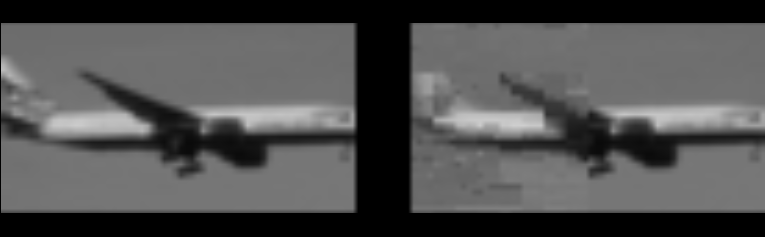
\includegraphics[scale=0.25]{imgs/plane0.png}
    
\includegraphics[scale=0.25]{imgs/face0.png} \\
    
\includegraphics[scale=0.25]{imgs/stop0.png}
    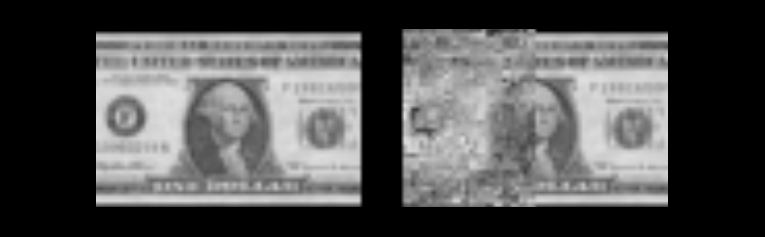
\includegraphics[scale=0.25]{imgs/dollar0.png}
    \caption{Image completion output from SPNs.}
  }
\end{figure}

Poon and Domingos also conducted preliminary experiments on object recognition. They ran
classification on three classes (one vs\. the other two) against convolutional DBNs (CDBNs). SPNs
showed almost flawless results.

\begin{table}[h]
  \centering{\captionsetup{justification=centering}
    \begin{tabular}{l | r | r | r}
      Architecture & Faces & Motorbikes & Cars \\
      \hline
      SPN & 99\% & 99\% & 98\% \\
      CDBN & 95\% & 81\% & 87\% \\
    \end{tabular}
    \caption{Comparison between CDBN and SPN on object recognition.}
  }
\end{table}

More information can be found on Poon and Domingos \textit{Sum-Product Networks: A New Deep
Architecture}~\cite{poon-domingos} and \textit{Learning the Structure of Sum-Product Networks}
\cite{gens-domingos}.

\newpage

\section{Structure of Sum-Product Networks}

In this section we work on the ideas presented in the previous sections. We will base this section
on the works of Poon and Domingos on their article \textit{Sum-Product Networks: A New Deep
Architecture}~\cite{poon-domingos} and also on Gens and Domingos' \textit{Learning the Structure of
Sum-Product Networks}~\cite{gens-domingos}.

\subsection{Partition function}

Probabilistic graphical models represent distributions compactly through a normalized product of
factors.

\begin{equation*}
  P(X=x) = \frac{1}{Z}\prod_k \phi_k (x_{\{k\}})
\end{equation*}

This equation states that the probability of $X$ taking value $x$ is the product of all factors,
with each factor taking a subset of the variables, divided by a partition function. The partition
function is the result of all the product of factors summed out.

\begin{equation*}
  Z = \sum_{x\in \mathcal{X}} \prod_k \phi_k(x_{\{k\}})
\end{equation*}

However, this form cannot represent all distributions. Additionally, inference is exponential in
scope size in the worst-case and learning takes sample size and time exponential. This is because
the partition function $Z$ is the sum of an exponential number of terms, and since all marginals
are sums of these terms, if $Z$ is tractable, then marginals are also tractable.

In Domingos and Poon~\cite{poon-domingos}, they claim that, since ``$Z$ is computed using only two
types of operations sums and products'', then ``it can be computed efficiently if $\sum_{x\in
\mathcal{X}} \prod_k \phi_k (k_{\{k\}})$ can be reorganized using the distributive law into a
computation involving only a polynomial number of sums and products.'' From this idea, they
elaborate on Darwiche's network polynomial and introduce Sum-Product Networks, a representation
that seeks to admit an efficient form for $Z$ whilst still being general.

\subsection{Definition}

Now we define a sum-product network formally.

\begin{spn-def}
  A sum-product network (SPN) is an acyclic digraph. An SPN $S$ over variables $X_1,\ldots,X_n$ has
  leaves as indicators $x_1,\ldots,x_n,\overline{x}_1,\ldots,\overline{x}_n$ and internal nodes as
  sums and nodes in alternating layers. For each edge $(i,j)$ that emanates from a sum node $i$,
  there exists a non-zero weight $w_{ij}$. The value of a sum node $i$ is $\sum_{j\in Ch(i)}
  w_{ij}v_j$, where $Ch(i)$ is the set of children of $i$ and $v_j$ is the value of the node $j$.
  The value of a product node $i$ is $\prod_{j\in Ch(i)} v_j$. The value of an SPN is the value of
  its root.
\end{spn-def}

\begin{figure}[h]
  \captionsetup{justification=centering}
  \centering{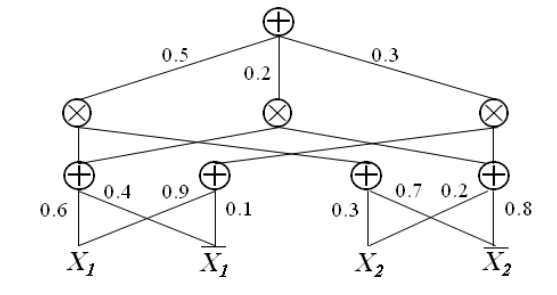
\includegraphics[scale=0.35]{imgs/spn_1.png}
    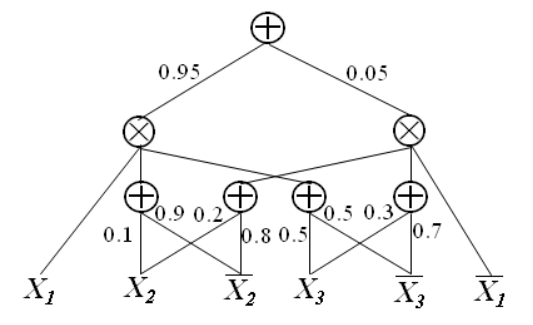
\includegraphics[scale=0.35]{imgs/spn_2.png}
    \caption{Two sum-product networks. The one on the left implements a naive Bayes mixture model
      and the other implements a junction tree. Note that the graph is shown as undirected, but it
      is in fact directed. All edges go from top to bottom. This is a choice of notation and may
      vary.}
  }
\end{figure}

An SPN $S$ as a function of the indicator variables $x_1,\ldots,x_n,\overline{x}_1,\ldots,
\overline{x}_n$ will be denoted by $S(x_1,\ldots,x_n,\overline{x}_1,\ldots,x_n)$. A complete state
$x$ means that, for each variable $X_i$, there are two possible outcomes for the indicators: either
$x_i=1,\overline{x}_i=0$ or $x_i=0,\overline{x}_i=1$. When an SPN $S$ has a complete state $x$,
instead of enumerating each indicator, we simply abbreviate to $S(x)$. $S(e)$ will be used to
denote when the indicators are specified according to the evidence $e$.

A sum-product network is an elaboration on Darwiche's network polynomial. We can look at an SPN as
a way to graphically represent the network polynomial of the distribution.

The partition function is the value of the network polynomial when all indicators are set to 1.
That is, $Z=\Phi(\mathbf{e})$ when $\mathbf{e}=\emptyset$. If an SPN $S$ has all indicators set to
1, we refer to it as $S(*)$. As we will see later, if an SPN $S$ is valid, then $S(*)=Z_S$.

The probability of evidence, $P(e)=\Phi(e)/Z$, is linear in the size of the network polynomial,
which in turn is exponential in the number of variables. However, it is possible, with a
sum-product network, to represent and evaluate the probability of evidence in space and time
polynomial.

SPNs are defined recursively, since the subnetwork at an arbitrary node $n$ in an SPN is an SPN\@.
We will denote an SPN rooted at node $n$ as $S_n(\cdot)$. Let $\mathbf{X}$ be the set of variables
in an SPN $S$, then for all $x\in \mathbf{X}$ the values of $S(x)$ define an unnormalized
probability distribution over $\mathbf{X}$. The unnormalized probability of evidence $e$ of an SPN
$S$ is given by $\Phi_S(e)=\sum_{x\in e}S(x)$, where the sum is over states consistent with $e$.
The $Z$ partition function of a distribution defined by $S(x)$ is $Z_S=\sum_{x\in \mathbf{X}}S(x)$.
The scope of an SPN $S$ is the set of variables that appear in $S$. A variable $X_i$ is negated in
$S$ if $\overline{x}_i$ is a leaf and non-negated if $x_i$ is a leaf.

The normalized probability distribution of an SPN $S_n$ is given by $P(x)=S_n(x)/Z_n$. If all
weights in the SPN $S$ are values $[0,1]$, then $Z_n=1$ and $S_n(x)$ is the probability
distribution.

Taking the left SPN in Figure 1 as an example, we have the value of the SPN as:

\begin{align*}
  S(x_1,x_2,\overline{x}_1,\overline{x}_2)=&\phantom{{} +{}}0.5(0.6x_1+0.4\overline{x}_1)(0.3x_2+0.7\overline{x}_2)+\\
                                           &+0.2(0.6x_1+0.4\overline{x}_1)(0.2x_2+0.8\overline{x}_2)+\\
                                           &+0.3(0.9x_1+0.1\overline{x}_1)(0.2x_2+0.8\overline{x}_2)
\end{align*}

The network polynomial is then:

\begin{equation*}
  \Phi = (0.5\times0.6\times0.3+0.2\times0.6\times0.2+0.3\times0.9\times0.2)x_1x_2+\ldots
\end{equation*}

If we have a complete state $x$ as $X_1=1,X_2=0$ then $S(x)=S(1,0,0,1)$, with indicators replaced
with their respective value. If the evidence $e$ is $X_1=1$, then, following the consistency rule,
we have that $S(e)=S(1,1,0,1)$. And as we have seen before, $S(*)=S(1,1,1,1)$.

\section{Properties of Sum-Product Networks}

We will now discuss a few properties described in Poon and Domingos' \textit{Sum-Product Networks:
A New Deep Architecture}~\cite{poon-domingos} and Gens and Domingos' \textit{Learning the Structure
of Sum-Product Networks}~\cite{gens-domingos}.

We first introduce two properties: completeness and consistency. Then we define validity, a
property that guarantees exact inference in time linear to the size of the SPN's edges. After that
we discuss tractability of the partition function, decomposability and we show that the partition
function, the probability of evidence and the MAP fo the SPN can be computed in time linear to the
size of the SPN if it is valid.

\subsection{Completeness and consistency}

Let us define the two properties:

\begin{spn-def}
  A sum-product network is complete iff all children of the same sum node have the same scope.
\end{spn-def}

What this definition says is that, the children of a sum node must all be from the same variable.
The trivial case is when all the children of the sum node $i$ are leaves. If $S_i$ is complete,
then all leaves are indicators of a same variable. This is easily extended to the general case,
since if, given a sum node $j$, all $Ch(j)$ are complete then all $S_k\in Ch(j)$ are complete and
thus $S_j$ is complete. If there exists an $S_k\in Ch(j)$ that is incomplete, then $S_j$ is
incomplete.

\begin{figure}[h]
  \centering{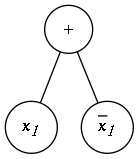
\includegraphics[scale=0.5]{imgs/complete.png}
    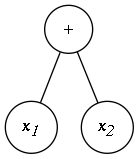
\includegraphics[scale=0.5]{imgs/incomplete.png}
    \captionsetup{justification=centering}
    \caption{On the left a complete SPN\@. On the right an incomplete SPN\@.}
  }
\end{figure}

\begin{spn-def}
  A sum-product network is consistent iff no variable appears negated in one child of a product
  node and non-negated in another.
\end{spn-def}

This means that product nodes take different variables and multiply them together. A variable $X_i$
is negated if there exists a leaf $\overline{x}_i$ on the SPN\@. It is non-negated if there exists
a leaf $x_i$. Therefore, if an SPN $S_k$ has a variable $X_i$ and is consistent, then for all
leaves of $S_k$, the presence of $x_i$ and $\overline{x}_i$ is mutually exclusive. That leads to
the fact that if an SPN $S_p$ has an inconsistent sub-SPN $S_q$, then $S_p$ is inconsistent.

\begin{figure}[h]
  \centering{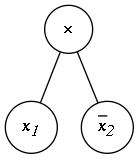
\includegraphics[scale=0.5]{imgs/consistent.png}
    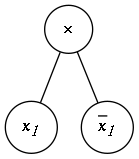
\includegraphics[scale=0.5]{imgs/inconsistent.png}
    \captionsetup{justification=centering}
    \caption{On the left a consistent SPN\@. On the right an inconsistent SPN\@.}
  }
\end{figure}

If an SPN is consistent but incomplete, it does not include monomials that should be present in the
network polynomial. This is

\subsection{Validity}

\section{Inference on Sum-Product Networks}

\subsection{Marginals}

\subsection{Most probable explanation (MEP)}

\section{Learning Sum-Product Networks}

\subsection{Learning the weights}

\subsection{Learning the structure}

\newpage
\begin{appendices}
\section{Notation}\label{app:not}

In this section we show the notations we use throughout this paper.

\subsection{Letters}

We use an uppercase letter to denote a variable. A lowercase letter denotes an instance of a
variable. A bold fonted letter is a set. A bold fonted uppercase letter is a set of variables. For
instance:

\begin{equation*}
  \mathbf{X}=\{X_1=x_1,\ldots,X_n=x_n\}
\end{equation*}

When dealing with indicator variables, the indicator function will be abbreviated as a lowercase
letter. That is, $[X_i]$ will be abbreviated to $x_i$. Similarly, $[\overline{X}_i]$ will be
written as $\overline{x}_i$. This clearly contradicts our first notation rule, however the two
meanings will be clear from context and therefore conflicts will never occur.

\subsection{Events and evidence}

The letter `e', regardless of case, is reserved for events and evidence. An uppercase `$E$' is an
evidence variable. An uppercase bold fonted `$\mathbf{E}$' is the set of evidence variables. A
lowercase `$e$' is a particular observed event variable. A bold fonted lowercase `$\mathbf{e}$' is
the set of variables of a particular observed event.

\subsection{Probabilities}

All functions of the form $P(\cdot)$ are probability functions. Joint probability distributions
have the variables separated by commas $P(X,Y)$ instead of $P(X \wedge Y)$. We call prior
probabilities the probability functions of the form $P(X)$. Posterior probabilities are of the form
$P(\mathbf{X}|\mathbf{Y})$.

When enumerating a set of instances we may omit commas, brackets or set name. For instance:

\begin{align*}
  &P(\mathbf{X}=a\overline{b}c) \text{~is equivalent to} \\
  &P(\mathbf{X}=\{a, \overline{b}, c\}) \text{~is equivalent to} \\
  &P(a\overline{b}c) \text{~is equivalent to} \\
  &P(a=true,b=false,c=true)
\end{align*}

\subsection{Arrows}

An arrow pointing to the right may have two possible meanings:

\begin{itemize}
  \item Dependency
    \begin{itemize}
      \item $A \to B$ is read as \textit{B depends on A}.
    \end{itemize}
  \item Directed edge connectivity
    \begin{itemize}
      \item $A \to B$ is read as \textit{there exists an edge from node A to node B}.
    \end{itemize}
\end{itemize}

Meanings will be clear from context.

\section{Mathematical background}\label{app:bak}

\end{appendices}

\newpage

\printbibliography[heading=bibintoc]

\end{document}
